%%%%%%%%%%%%%%%%%%%%%%%%%%%%%%%%%%%%%%%%%%%%%%%%%%%
%
%  New template code for TAMU Theses and Dissertations starting Fall 2012.  
%  For more info about this template or the 
%  TAMU LaTeX User's Group, see http://www.howdy.me/.
%
%  Author: Wendy Lynn Turner 
%	 Version 1.0 
%  Last updated 8/5/2012
%
%%%%%%%%%%%%%%%%%%%%%%%%%%%%%%%%%%%%%%%%%%%%%%%%%%%
%%%%%%%%%%%%%%%%%%%%%%%%%%%%%%%%%%%%%%%%%%%%%%%%%%%%%%%%%%%%%%%%%%%%%%
%%                           SECTION V
%%%%%%%%%%%%%%%%%%%%%%%%%%%%%%%%%%%%%%%%%%%%%%%%%%%%%%%%%%%%%%%%%%%%%


\chapter{\uppercase{Experiments \& Results}}
To verify the idea proposed in this thesis, we setup environments, develop SAC framework and run some typical seismic applications on cluster in PVAMU cloud computing lab. There are three main layers in SAC: low-level runtime envrionment, SAC framework as middleware and application development interface at up-level. 

\section{Experiments Environment Setup}

The cluster used for conducting experiments consists of 26 nodes, in which one is management node, another is storage node used for managing disk array and other 24 nodes are computation nodes. Each node in such cluster was equipped with Intel Xeon E5-2640 Sandy Bridge CPU (2.5GHz, 12 Cores or 24 Cores with Hyperthreading support), 64GB DDR3 memory and are inter-connected with 1GB ethernet. Each node has its own local disk, and also could access disk array through NFS. Following the architecture stated in previous charpter, we install CentOS 6.5 (Distributed by Redhat) and Oracle JDK 1.8.0\_40 on each node. Hadoop 2.2.0, Spark 1.2.1 and other related libraries are installed on each node. In configuration of Hadoop, management node was configured as NameNode and other 24 computation nodes as DataNodes. It is similiar in Spark: management node is Master and other computation nodes are Workers. Cassandra was installed on all 24 computation nodes and the first four nodes was selected as seed nodes.


The public sample seismic dataset Penobscot \cite{PenobscotData} was selected as experiment data. The original format of Penobscot dataset is SEGY, and to make it easily processed with Spark, we transfer it into two files: one xml file that saves meta data, and aonther 3D data file with dimension size of 600x481x1501 stores actual data samples. The volume size of original data file is about 1.7GB, which is not big enough comaring with data set currently used in oil\&gas industry, so we use it synthesize a new 100GB file for verifying algorithms and models on SAC. Both xml file and data file are stored on HDFS, so that every node could access them and utilize data locality. The intermediate results are stored in Cassandra basing on requirement and final result are persisted on HDFS. 

\section{Application Development Platform}


%%%%%%%%%%%%%%%%%%%%%%%%%%%%%%%%%%%%%%%%%%%%%%%%%%%%%%%
\begin{figure}[H]
\centering
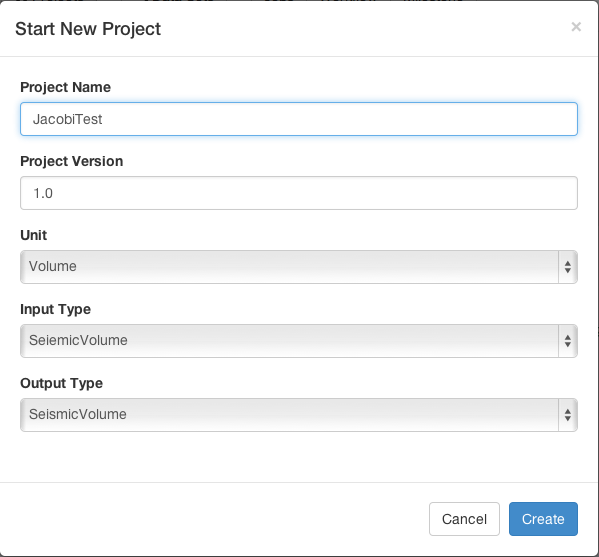
\includegraphics[scale=.60]{figures/NewProject.png}
\caption{Configure Template on Creating New Project}
\label{NewProject}
\end{figure}
%%%%%%%%%%%%%%%%%%%%%%%%%%%%%%%%%%%%%%%%%%%%%%%%%%%%%%%

%%%%%%%%%%%%%%%%%%%%%%%%%%%%%%%%%%%%%%%%%%%%%%%%%%%%%%%
\begin{figure}[H]
\centering
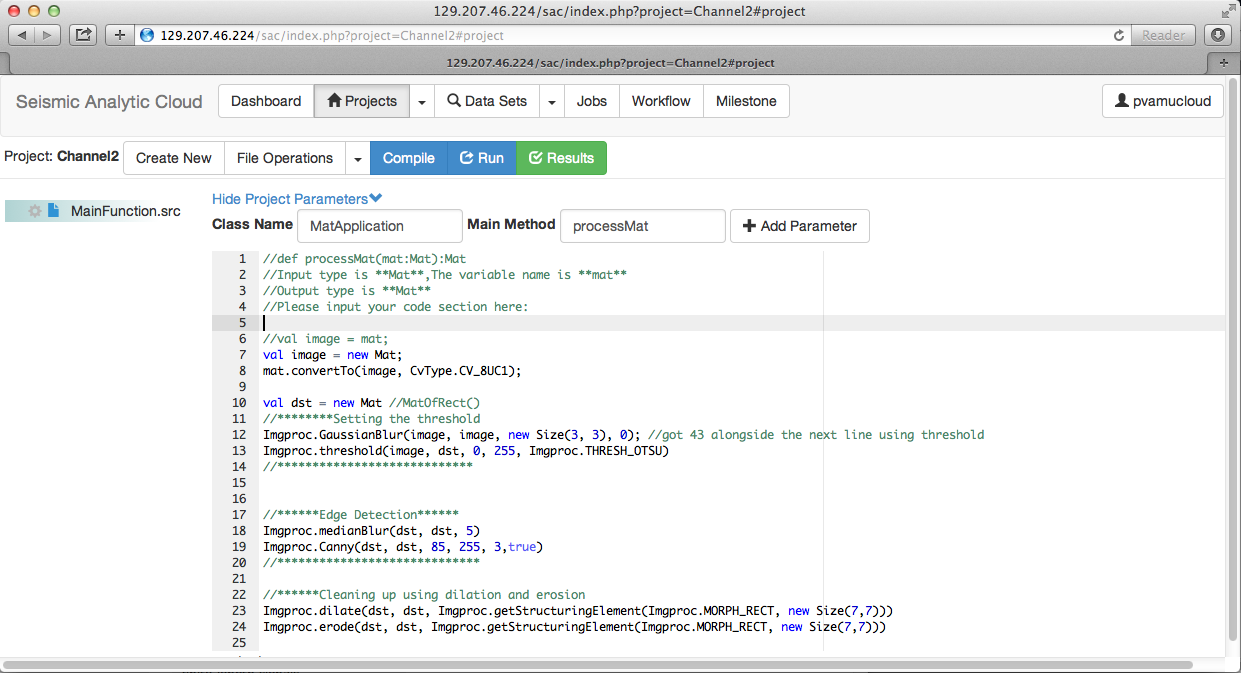
\includegraphics[scale=.35]{figures/Programming.png}
\caption{Programming and Running on Web Interface}
\label{Template}
\end{figure}
%%%%%%%%%%%%%%%%%%%%%%%%%%%%%%%%%%%%%%%%%%%%%%%%%%%%%%%


%%%%%%%%%%%%%%%%%%%%%%%%%%%%%%%%%%%%%%%%%%%%%%%%%%%%%%%
\begin{figure}[H]
\centering
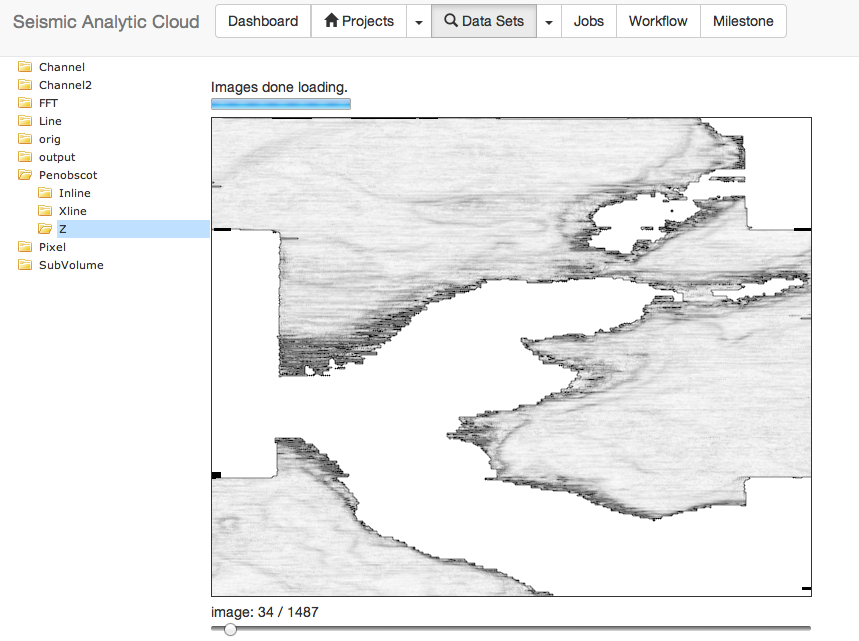
\includegraphics[scale=.45]{figures/DataSet.png}
\caption{Seismic Dataset Preview}
\label{Template}
\end{figure}
\subsection{Subsection}
%%%%%%%%%%%%%%%%%%%%%%%%%%%%%%%%%%%%%%%%%%%%%%%%%%%%%%

%A table example is going to follow.
%\begin{table}[H]
%\centering
%\caption{This is a table template}
%\begin{tabular}{|l|c|c|c|c|c|}
%\hline
%Product & 1 & 2 & 3 & 4 & 5\\
%\hline
%Price & 124.- & 136.- & 85.- & 156.- & 23.-\\
%Guarantee [years] & 1 & 2 & - & 3 & 1\\
%Rating & 89\% & 84\% & 51\% & & 45\%\\
%\hline
%\hline
%Recommended & yes & yes & no & no & no\\
%\hline
%\end{tabular}
%\label{tab:template2}
%\end{table}
%\subsubsection{This is a subsubsection}
%%%%%%%%%%%%%%%%%%%%%%%%%%%%%%%%%%%%%%%%%%%%%%%%%%%%%%

\section{Case Study}


\subsection{Caclulator}




\subsection{Filter \& Transformation}



\subsection{Complicate Stencil Operation}





